\let\negmedspace\undefined
\let\negthickspace\undefined
\documentclass[journal]{IEEEtran}
\usepackage[a5paper, margin=10mm, onecolumn]{geometry}
%\usepackage{lmodern} % Ensure lmodern is loaded for pdflatex
\usepackage{tfrupee} % Include tfrupee package

\setlength{\headheight}{1cm} % Set the height of the header box
\setlength{\headsep}{0mm}     % Set the distance between the header box and the top of the text

\usepackage{gvv-book}
\usepackage{gvv}
\usepackage{cite}
\usepackage{amsmath,amssymb,amsfonts,amsthm}
\usepackage{algorithmic}
\usepackage{graphicx}
\usepackage{textcomp}
\usepackage{xcolor}
\usepackage{txfonts}
\usepackage{listings}
\usepackage{enumitem}
\usepackage{mathtools}
\usepackage{gensymb}
\usepackage{comment}
\usepackage[breaklinks=true]{hyperref}
\usepackage{tkz-euclide} 
\usepackage{listings}
% \usepackage{gvv}                                        
\def\inputGnumericTable{}                                 
\usepackage[latin1]{inputenc}                                
\usepackage{color}                                            
\usepackage{array}                                            
\usepackage{longtable}                                       
\usepackage{calc}                                             
\usepackage{multirow}                                         
\usepackage{hhline}                                           
\usepackage{ifthen}                                           
\usepackage{lscape}
\begin{document}

\bibliographystyle{IEEEtran}
\vspace{3cm}

\title{CHAPTER - 9\\Differential Equations}
\author{EE24BTECH11061 - Rohith Sai}
% \maketitle
% \newpage
% \bigskip
{\let\newpage\relax\maketitle}

\renewcommand{\thefigure}{\theenumi}
\renewcommand{\thetable}{\theenumi}
\setlength{\intextsep}{10pt} % Space between text and floats

\numberwithin{figure}{enumi}
\renewcommand{\thetable}{\theenumi}

\section*{Exercise : 9.5}
\begin{enumerate}
\item [9)] Solve the differential equation $y \, dx + x \log{\brak{\frac{y}{x}}} \, dy - 2x \, dy = 0$ \\
\textbf{Solution (using the Method of Finite Differences):}\\
The given differential equation is 
\begin{align}
    y \, dx + x \log{\brak{\frac{y}{x}}} \, dy - 2x \, dy = 0
\end{align}
\begin{align}
y \, dx &= \left(2x - x \log\left(\frac{y}{x}\right)\right) \, dy \\
\implies \frac{dx}{dy} &= \frac{2x - x \log\left(\frac{y}{x}\right)}{y} \\
\implies \frac{dy}{dx} &= \frac{\frac{y}{x}}{2 - \log\left(\frac{y}{x}\right)} 
\end{align}

Using the method of finite differences, the next value of $y$ can be computed as:

\begin{align}
y_{n+1} &= y_n + h \cdot f(x_n, y_n) \\
f(x, y) &= \frac{\frac{y}{x}}{2 - \log\left(\frac{y}{x}\right)}
\end{align}

Let $x_0$ be the initial $x$ value and $y_0$ be the initial value and let the step size $h$ be 0.001. The first few iterations are:

\begin{align*}
x_1 &= x_0 + h, & y_1 &= y_0 + h \cdot \frac{\frac{y_0}{x_0}}{2 - \log\left(\frac{y_0}{x_0}\right)} \\
x_2 &= x_1 + h, & y_2 &= y_1 + h \cdot \frac{\frac{y_1}{x_1}}{2 - \log\left(\frac{y_1}{x_1}\right)} \\
&\vdots  & \vdots \\
x_n &= x_{n-1} + h, & y_n &= y_{n-1} + h \cdot \frac{\frac{y_{n-1}}{x_{n-1}}}{2 - \log\left(\frac{y_{n-1}}{x_{n-1}}\right)}
\end{align*}

\textbf{Solution (using the general method):}\\
Let $\frac{y}{x} = v$, i.e., $y = vx$
\begin{align*}
    \implies \frac{dy}{dx} = v + x \frac{dv}{dx}
\end{align*}
Substituting in equation (4), we get:
\begin{align*}
    v + x \frac{dv}{dx} = \frac{v}{2 - \log{v}}\\
    \implies x \frac{dv}{dx} = \frac{v}{2 - \log{v}} - v\\
    \implies x \frac{dv}{dx} = \frac{v \brak{\log{v} - 1}}{2 - \log{v}}\\
    \implies \frac{dx}{x} = \sbrak{\frac{1}{v \brak{\log{v} - 1}} - \frac{1}{v}} dv
\end{align*}
Integrating on both sides, we get:
\begin{align*}
    \log{\abs{x}} + \log{\abs{c}} = \int \sbrak{\frac{1}{v \brak{\log{v} - 1}} - \frac{1}{v}} dv\\
    \implies \log{\abs{x}} + \log{\abs{c}} = \log{\abs{\log{v} - 1}} - \log{\abs{v}}\\
    \implies C x v = \log{v} - 1 \quad \sbrak{\text{where, }C = \pm c} 
\end{align*}
Replacing $v$ by $\frac{y}{x}$ and rearranging, we have:
\begin{align*}
    \log{\brak{\frac{y}{x}}} - 1 = C x \brak{\frac{y}{x}}
\end{align*}
\begin{align}
    \log{\brak{\frac{y}{x}}} - 1 = C y 
\end{align}
Let's assume, $C=-1$ and $x = 1$. On substituting these values in equation (7), we get, $y = 1$.\\
Therefore, the equation is as follows:
\begin{align*}
    y = x e^{\brak{1-y}}
\end{align*}
Therefore, the curve generated using both the above mentioned methods for the given differential equation (1) is shown below:
\begin{figure}[H]
    \centering
    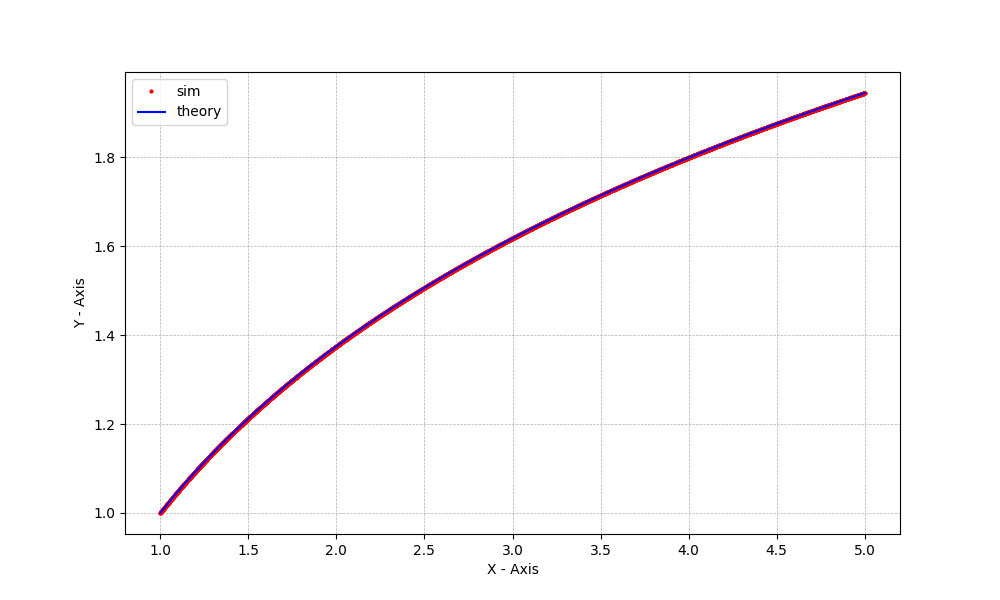
\includegraphics[width = \columnwidth]{figs/fig.png}
\end{figure}
\end{enumerate}
\end{document}